\newpage
\topskip0pt
\vspace*{\fill}
\section*{Abstract}
Trade-offs in performance of different ecological functions within a species are  commonly offered as an explanation for coexistence in natural communities. Single trade-offs between competitive ability and other life history traits have been shown to support a large number of species, as a result of strong competitive asymmetry. We consider a single competition-fecundity trade-off in a homogeneous environment, and examine the effect of the form of asymmetry on the likelihood of species coexisting. We find conditions that allow coexistence of two species for a general competition function, and show that (1) two species can only coexist if the competition function is sufficiently steep when the species are similar; (2) when competition is determined by a linear function, no more than two species can coexist; (3) when the competition between two individuals is determined by a discontinuous step function, this single trade-off can support an arbitrarily large number of species. Further, we show analytically that as the degree of asymmetry in competition increases, the probability of a given number of species coexisting also increases, but note that even in the most favourable conditions, large numbers of species coexisting along a single trade-off is highly unlikely. On this basis we suggest it is unlikely that single trade-offs are able to support high levels of biodiversity without interacting other processes.
\vspace*{\fill}
\newpage

\section{Introduction}


There is no such thing in the natural world as a Darwinian Demon which maximises all possible life history traits \citep{law1979optimal}, and instead individuals have to allocate resources to one life-history trait at the expense of others. This results in trade-offs between life history traits, so that, for example, a plant species which allocates resource to rapid growth does so at the expense of its ability to withstand shading; or a species that has allocated much of the available resource to out-competing other species will suffer a decrease in its ability to disperse and colonise empty areas of the environment  \citep[e.g.][]{tilman1994competition, cadotte2006testing}. Other classic life-history trade-offs include the offspring size-number trade-off \citep[e.g.][]{venable1992size}; the trade-offs between pathogen resistance and fecundity \citep[e.g.][]{bowers1994life}; and competition and intra-guild predation \citep{amarasekare2007trade}.

Theory has shown that these trade-offs can allow two or more species to coexist while competing for the same resources  \citep[e.g.][]{kisdi2003coexistence, levins1971regional, bonsall2004life}, and consequently that trade-offs may be instrumental in the evolution of biodiversity \citep{schluter1995adaptive, white2005adaptive, bonsall2004life}. In particular, \cite{levins1971regional} originally highlighted two such trade-offs, the competition-colonisation trade-off which has received much attention, and the trade-off between death rate and competitive ability which has received less attention. Levins and Culver argued that two species can coexist if one experiences a lower death rate, but is a weaker competitor than the other species. Both trade-offs are closely related, and have received much attention, with \cite{tilman1994competition} showing that the competition-colonisation trade-off can potentially lead to infinitely many species coexisting.

However, the conditions under which species either competitively exclude, or coexist alongside others due to trade-offs between competition and other life history traits might also be dependent on the existence, and level, of asymmetric competition between species \citep{adler2000space}. Competition is called asymmetric if an individual with larger trait value (e.g. size) is bestowed some benefit over small trait valued neighbours, winning more than 50\% of contests by virtue of this difference in trait. This competition is deemed to be very asymmetric if there is a large difference in competitive ability between individuals which have slightly different trait values. Asymmetric competition is widespread in the natural world, forming the majority of inter-species competition in insects \citep{lawton1981asymmetrical}; and is prevalent in plants where competition for light is expected to be size dependent, such that a larger plant may intercept nearly all the available light at the expense of a smaller individual \citep{weiner1990asymmetric}. However, there is relatively little theory that investigates how the strength of competitive asymmetry may affect the maintenance of biodiversity.

\cite{adler2000space} demonstrated that, if the competition between two species is determined by a step function with infinite gradient when traits are the same, then the species richness, the number of species present in the community, is maximised in their model. They then used numerical simulations of their model to show how reducing the degree of competitive asymmetry reduces the number of species that can coexist on the trade-off. Similarly,  \cite{kisdi1999evolutionary} showed that the gradient of the competition function at the point where two competing individuals have the same trait value (i.e. the same size), is critical in determining the number of species that may evolve in the long term. In other words, coexistence and the evolution of a large community seem to be more likely if a small change in fecundity translates into a large change in competitive ability.

Here we build on this  previous work and analyse a model with a single trade-off between competitive ability and fecundity. We will find conditions required for two species to coexist, and demonstrate that while no more than two species can coexist when competition is a linear function of the trait value, if the mechanisms of the competition between species allows for a discontinuity in the competition function, then coexistence of any number of distinct species is possible. We also demonstrate analytically for two species that this discontinuous competition gives an upper bound on the likelihood of coexistence when compared with two convex-concave functions that tend to the step function as parameters are altered. Niche theory suggests that as species become more similar coexistence should become more unlikely, but few studies have quantitatively investigated this in the context of life-history trade-offs. Using rigorous proofs we will show that competitive asymmetry and the gradient of the competition function at the origin are important in determining the number of species able to persist on one trade-off, but also show that even under the most favourable conditions, large numbers of species coexisting on one trade-off is very unlikely.
 
\section{The Model}

We examine coexistence criteria in a simple model where species differ only in their per capita fecundity and their competitive ability. The per capita fecundity is compared to competitive ability through assigning a trait value to each species. The typical traits we have in mind are body size, or weight of armament, and a strong competitor has a lower fecundity, creating a competition-fecundity trade-off. In doing so we assume a species which is a stronger competitor diverts resources into this trait, perhaps by delaying reproduction and growing in size; whereas a weaker competitor diverts more resources into reproduction at the cost of competitive ability. We assume this trade-off, which restricts parameter space within the model, is conserved across species, and that it can be described by two functions that relate a species' trait value to (i) fecundity, and (ii) competitive ability. In particular, we will explore how the shape of the latter function is important in determining the amount of species that may be supported by the trade-off.


Let $n$ denote the number of species present in the environment, with species $i$ having expected size $x_i$ and population density $N_{x_i}$. We use Lotka-Volterra equations to describe the population dynamics:
 \begin{equation}
\label{model}
 \frac{d N_{x_i}}{dt}=N_{x_i}\left( p(x_i) - \sum_{j=1}^n c(x_i - x_j)N_{x_j}\right),
 \end{equation}
where $p(x_i)$ is the intrinsic growth rate of species $i$ when resources are not limiting and the environment is free of competition;  $c(x_i-x_j)$ is the competition kernel used to quantify the impact of competition with species $j$ on species $i$ which depends only on the difference in trait values $x_i-x_j$. For larger species, which have lower fecundity, $p(x_i)$ is lower than for species with smaller trait values, so we assume that  $p(x_i)$ is a strictly decreasing non-negative function of trait value  $x_i$. The intrinsic growth rate $p$ is assumed to be greater than zero, as any species with a non-positive growth rate would not be able to grow in even an empty environment. Since we are at liberty to choose units for $x$, we choose $x_{max}=1$ since the maximum trait value for which the growth rate is zero: $p(1)=0$. Similarly, we let $x_{min}=0$ be the smallest permissible trait value, meaning all extra resources are diverted into fecundity rather than competitive ability. In what follows we will mainly work with the linear growth function  $p(x_i)=\rho(1- x_i)$ where $\rho>0$. However, we will use $ p(x_i)$ wherever possible in order to show how the method may be extended to nonlinear growth functions. Using these assumptions, our aim is to investigate the possibility and probability of coexistence of species selected at random across the entire trait-space.

The continuous competition kernels $c(x_i - x_j)$ we consider are non-increasing functions of the difference between the individual's trait value and that of its competitor, i.e. non-increasing in $(x_i-x_j)$. This means that an individual with large trait value experiences little competition from competing individuals with smaller trait values, while small trait value individuals suffer a much larger competitive effect from large individuals. For example, taller trees will clearly intercept light earlier than shorter individuals, while shading shorter neighbours. However, shorter trees will have limited shading effect on a tall neighbour. We use convex-concave functions, to reflect the realistic assumption that two large species will have a similar effect on a much smaller third species, while a large individual will suffer approximately equal effects from two much smaller individuals. However, when all three species are of similar size, the effects of the larger (smaller) two on the smallest (largest) may vary significantly. The discontinuous competition is a suitable limit of such continuous functions, and although it is less realistic, it allows for useful analytical upper bounds for the continuous cases.

We study the effects of asymmetric competition for two species considering (1) a general function $c(z)$ and linear growth, with a focus on two examples; and (2) for general growth  $p(x_i)$ with linear and step function $c(x_i - x_j)$, which we also consider for $n>2$. As with the growth function, the general linear competition kernel is studied, with
 \begin{equation}
 \label{linearc}
 c(x_i - x_j)=\kappa - \theta (x_i - x_j),
 \end{equation}
but additional restrictions are applied to the convex-concave and step functions model. To ensure that the effect of this competition is never positive, such that the model represents a predator-prey interaction or mutualism, it is necessary to have $\kappa>\theta$. The intraspecific competition (i.e. when $x_i=x_j$) is assumed to be identical across species, and can be scaled to one to reduce the number of parameters, and it is assumed that the total negative effect of competition in an interaction between any two individuals is the same. Ecologically, this means that there is a set amount of resource to be shared between any two individuals. When the two individuals are the same species and have equal trait values, each takes on average 50\% of the resource, or wins the competitive contest roughly half of the time. When the trait values differ, the stronger competitor takes a greater percentage of the resource, leaving less for the weaker competitor. To reflect this we study two continuous competition functions, a piecewise linear function given by 
\begin{equation}
\label{pwlcomp}
c(x_i-x_j)=\begin{cases}
1+\epsilon & x_i-x_j\leq-\Theta \\
1-\frac{\epsilon}{\Theta}(x_i-x_j) & -\Theta<x_i-x_j<\Theta \\
1-\epsilon & x_i-x_j >\Theta, 
\end{cases}
\end{equation}
and a smooth function modified from that used by Kisdi \cite{kisdi1999evolutionary}, which we consider as
\begin{equation}
\label{kisdimodified}
c(x_i-x_j)=1+\epsilon -\frac{2\epsilon}{1+e^{-\frac{2(x_i-x_j)}{\Theta}}}.
\end{equation}
As $\Theta$ tends to zero, these two functions both tend to a step function, that will be considered in detail for general $n$ species dynamics. This  function is given by
 \begin{equation}
 \label{stepc}
 c(x_i - x_j)=\begin{cases}
 1+\epsilon & x_i <x_j \\
 1 & x_i = x_j \\
 1-\epsilon & x_i > x_j
 \end{cases},
 \end{equation}
and is used as the discontinuous competition function throughout this study (see also \cite{tilman1994competition, may1994superinfection}).
 
Our model is similar to those studied by \cite{law1997evolution} and \cite{kisdi1999evolutionary}, although both of their models only considered a concave-convex competition function in lieu of the linear and discontinuous functions considered for large $n$ here. The function $c_{k,\nu}(z) =  c(1-1/(\nu+e^{kz}))$ used by Kisdi, of which \eqref{kisdimodified} is a modified version tends to a discontinuous step function of the type studied here as $\theta = 1/k$ tends to zero ($\nu>0$ fixed). The use of simplified competition functions in this study allows for more analytical work than the more complex functions used in Kisdi's analysis. We demonstrate in the two species case that our results for the discontinuous competition function are similar to those produced using the competition kernel given by \eqref{kisdimodified} when $\theta$ is small, and hence allow for comparison with Kisdi's competition model which shows qualitatively similar results for two species coexistence with linear growth.

When $\epsilon=1$, our model with a step function $c(z)$ takes the same form as the spatially implicit model presented by Klausmeier \cite{klausmeier1998extinction}, which also demonstrates that coexistence is possible for general $n$. However, this current study builds upon this work to indicate both the likelihood of this coexistence, and the effects of weakened asymmetry in competition.

Before studying the effects of trade-offs on the coexistence of species, it is important to clarify what we mean by coexistence. In its strongest sense, coexistence can be taken to mean that all species present persist at a given positive equilibrium value. This means that any mathematical model of the system will exhibit coexistence if and only if there is a positive fixed point that is globally asymptotically stable, in the sense that all initial conditions for which each species has positive density end up at a positive equilibrium density. This is the notion of coexistence used by Strobeck \cite{strobeck1973n}. Law \cite{law1996permanence} uses a less stringent definition of coexistence, namely that the system exhibits coexistence if all species densities remain bounded and for all positive initial densities, there is a  density $\delta>0$ such that all the species eventually exceed $\delta$, demonstrated mathematically by the concept of permanence. In this study, a collection of species is considered to exhibit coexistence if the model of those species exhibits permanence. However, as permanence is an immediate consequence of a globally asymptotically stable equilibrium in the interior, the existence of the latter is used to show coexistence in our discontinuous competition model.

In later sections we study n-species communities and investigate the likelihood of coexistence given the model, and the trade-off function. Here we assume communities are assembled randomly from a regional species pool where all species (trait values) are present. We note that our results will be different to the expected number of species that will evolve via small mutations from a mono-specific community; or from community assembly by invasion of species one at a time; but in both cases relatively high levels of coexistence are required for large communities to occur.

\section{Results}

\subsection{Linear Competition}
Suppose that the competitive advantage held by one species over another is a linear function of the difference between the trait values of the two species. Then the competition coefficients $c(x_i -x_j)$ in \eqref{model} are determined by use of the function given in \eqref{linearc}. In order to preserve the competition-fecundity trade-off, it is necessary that as fecundity decreases - and the function $p(x_i)$  decreases - the competitive advantage that the species holds over a fixed, weaker competitor is increasing. This translates to the mathematical condition $\theta>0$. To simplify the calculations, it is assumed that $x_i>x_{i+1}$, but the results shown apply to any ordering of species, and therefore trait values. 
The equations for the two species system are
\begin{eqnarray*}
\frac{dN_{x_1}}{dt} & = & N_{x_1} \left\{ p(x_1) - \kappa N_{x_1} - (\kappa-\theta(x_1-x_2))N_{x_2} \right\}\\
\frac{dN_{x_2}}{dt} & = & N_{x_2} \left\{ p(x_2) - (\kappa-\theta(x_2-x_1))N_{x_1}-\kappa N_{x_2}\right\}.
\end{eqnarray*}

This model admits an interior fixed point when
\begin{equation}
\label{lin2dposfp}
 \frac{\kappa}{\theta}\frac{p(x_2)-p(x_1)}{p(x_2)}<x_1-x_2< \frac{\kappa}{\theta}\frac{p(x_2)-p(x_1)}{p(x_1)},
 \end{equation}
and this is globally stable  whenever it exists, since $\kappa>0$ by assumption. Therefore, coexistence is possible if the condition \eqref{lin2dposfp} is satisfied.

However, the limits of linear competition in giving rise to coexistence are shown if a third species is introduced to the system. We now demonstrate that regardless of the trait value this species holds, or the parameter values for $\kappa, \theta$, it cannot form a permanent three species system with the two already species present.  

Note that when equation \eqref{linearc} is used, the $3\times 3$ matrix of competition coefficients has a determinant of zero, i.e. is singular, and that therefore the model does not have a unique equilibrium point in the interior. In Lotka-Volterra systems, this means that the system does not exhibit permanence (Theorem 13.5.1 in \cite{hofandsig}).

Therefore, no third species can form a permanent coalition with the two species already present. We conclude that with a linear function for competition, a maximum of two species can stably coexist and when a third species is introduced, the model exhibits neither asymptotic stability nor permanence. The linear trade-off case is degenerate, but it is useful in illustrating the dependence of the model on the form of the competition function. We therefore switch our attention to a model utilising a nonlinear competition function.

\subsection{Generalised Competition in the two species case}
Consider a generalised competition function $c(x_i - x_j)=c(z)$, which is decreasing, such that $c�(z)\leq0$ for all $z$, for two species. These species are different in two aspects, competitive ability and population growth rate (effectively $K$ and $r$ respectively), both of which are determined by a single parameter $x_i$ for species $i$. We assume that growth rate decreases linearly with $x_i$, such that $x_i$ can be considered as the proportion of non essential resource dedicated to competitive strength at the expense of population growth rate. It is simple to scale the model such that we can define this growth rate by the function $p(x)=1-x$. This therefore means that competitive ability must increase with $x_i$ when the second species remains unchanged. We assume that the competition coefficients are a function of $x_1-x_2$, so therefore can be treated by a function $c(z)$ of a single variable $z$. The competition coefficient $c_{ij}$ gives the negative effect of species $j$ on species $i$, and is defined by $c(x_i-x_j)$. This means that $c(z)$ must be a monotonically decreasing function of $z$. Note the model can be scaled to ensure $c(0)=1$ without any loss of information. 

If two species have identical competitive ability, but differ in growth rate, then the faster growing species would competitively exclude the slower grower, so an essential condition for coexistence is that $c'(0) <0$. 
 
Therefore, the system is given by
\begin{equation}
 \dot{N_1}=N_1\left(1-x_1 -N_1-c(z)N_2\right),
\end{equation}
\begin{equation}
  \dot{N_2}=N_2\left(1-x_2 -N_2-c(-z)N_1\right).
  \end{equation}
  where $z=x_1-x_2$. The condition for global stability of an interior fixed point is then given by $c(z)c(-z)<1$, which is therefore a further condition on the function $c(z)$ for coexistence in the 2-species case.

It is simple to show that an interior fixed point is present when 
\begin{align}
1-x_1-c(z)(1-x_2)&>0, \\
1-x_2-c(-z)(1-x_1)&>0. \end{align}
By writing these as functions of $z$ and $x_2$, it is possible to rearrange to get
\begin{align}
\label{x2upper}
x_2&<\frac{1-z-c(z)}{1-c(z)} \\
\label{x2lower}x_2&>\frac{(1-z)c(-z)-1}{c(-z)-1} \end{align}
We now assume without loss of generality that species 1 is the competitively dominant species, i.e. $z>0$. Then if we define $z^*$ such that
$
1-z^*-c(z^*)=0$
and $\hat{z}$ such that
$1-(1-\hat{z})c(-\hat{z})=0,$
 (defined uniquely for convex-concave functions where $z c''(z)>0$ for $z\neq0$ and $c'(0)<-1$),
then the area of coexistence can be found by
\begin{equation}
\label{areacoexist}
2\left( \int^{z^*}_0 dz \frac{1-z-c(z)}{1-c(z)} - \int^{\hat{z}}_0 dz \frac{(1-z)c(-z)-1}{c(-z)-1} \right)
\end{equation}
where the factor of 2 is to include the other ordering of traits. It is relatively simple to show that with these assumptions, coupled with the fact that $c(-z)+c(z)=2$, coexistence is only possible if $c'(0)<-1$ (Appendix~\ref{appendix1a}). This is in accordance with the work of Adler and Mosquera, who state that monoculture will prevail when the steepness of the competition curve has magnitude less than 1.

As an example, we use the modified version of the function used by Kisdi \cite{kisdi1999evolutionary} given by \eqref{kisdimodified}, scaled such that the intraspecific competition coefficients are unity, and the parameter $\epsilon$ measured the greatest level of dominance possible, so $c(z) \in [1-\epsilon,1+\epsilon]$ for all $z$.  There is an issue in that $z^*$ and $\hat{z}$ as defined above cannot be found by simply rearranging these equations. However, as demonstrated in Figure~\ref{kisdipic}, when we numerically find the area of the region of coexistence, this area monotonically decreases as the parameter $\Theta$ is increased. The likelihood of coexistence is maximised at $\Theta=0$, where the competition coefficients are determined by a step function. Using Taylor series expansions of the functions $F_1(z)=1-z-c(z)$ and $F_2(z)=(1-z)c(-z)-1$, we can show that the area of coexistence tends to the results presented in Section 3.3 as $\Theta$ approaches 0.

\begin{figure}[htbp]
   \centering
   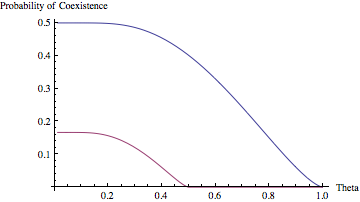
\includegraphics[width=4in]{kisdinum}
   \caption{How the probability of coexistence given by the convex-concave function \eqref{kisdimodified} changes with the parameter $\Theta$, which determines the steepness of the curve. Shown are the cases $\epsilon=1$ and $\epsilon=1/2$.}
   \label{kisdipic}
\end{figure}
 
As a further example, we can investigate the piecewise linear function \eqref{pwlcomp}, where pairs of species with similar trait values will have different effects on one another than pairs with different trait values, but that once a threshold of dissimilarity is passed, all species have the same effect on one another.  Note that this approximates the smooth function \eqref{kisdimodified} considered above. This gives two cases, as the function $(1-z)^{-1}$ will cross $c(-z)$ on the constant part for small $\Theta$, but the sloped part for slightly larger $\Theta$. The two cases are  that where $\Theta<\frac{\epsilon}{(1+\epsilon)}$ and that where $\frac{\epsilon}{(1+\epsilon)}<\Theta<\epsilon$. In the case where $\Theta$ is small, we can write the above integrals as
\[
2\left(\int_0^\Theta \frac{\epsilon-\Theta}{\epsilon}dz + \int_\Theta^{\epsilon} 1-\frac{z}{\epsilon}dz-\int_0^\Theta \frac{\epsilon-\Theta}{\epsilon}-z dz -\int_\Theta^{\frac{\epsilon}{1+\epsilon}} 1-\frac{1+\epsilon}{\epsilon}z dz\right)\]
\[= 2\left(\Theta-\frac{\Theta^2}{\epsilon}+\frac{\epsilon}{2}-\Theta+\frac{\Theta^2}{2\epsilon}-\Theta+\frac{\Theta^2}{\epsilon}+\frac{\Theta^2}{2}+\frac{\epsilon}{2(1+\epsilon)^2}+\frac{\epsilon^2}{2(1+\epsilon)^2}-\frac{\epsilon}{1+\epsilon}+\Theta-\frac{\Theta^2}{2}-\frac{\Theta^2}{2\epsilon}\right)\notag
\]
\[=\frac{\epsilon^2}{1+\epsilon}\]
For larger $\Theta$, we can write the integrals as
\[
2\left(\int_0^\Theta \frac{\epsilon-\Theta}{\epsilon}dz + \int_\Theta^{\epsilon} 1-\frac{z}{\epsilon}dz-\int_0^{\frac{\epsilon-\Theta}{\epsilon}} \frac{\epsilon-\Theta}{\epsilon}-z dz\right) \]
\[=2\left(\Theta-\frac{\Theta^2}{\epsilon}+\frac{\epsilon}{2}-\Theta+\frac{\Theta^2}{2\epsilon}-\frac{1}{2}+\frac{\Theta}{\epsilon}-\frac{\Theta^2}{2\epsilon^2}\right)\notag 
\]
\[
=\frac{(\epsilon-\Theta)(\Theta+\epsilon(\epsilon+\Theta-1))}{\epsilon^2}.
\]
We therefore find that the probability of two species coexisting is constant for small $\Theta<\epsilon/(1+\epsilon)$, and a decreasing function of $\Theta$ when the competitive difference between similar species is smaller, i.e. when $\Theta$ is larger. Because in both this in the concave-convex case, the step function limit serves to maximise the probability of two species coexisting, we now consider the discontinuous case in more detail, as this will give an upper bound on the probability of coexistence for $n$ species.

\subsection{Discontinuous Competition}
In a similar model to that presented here Adler and Mosquera \cite{adler2000space} demonstrated how species richness increases with the gradient of the competition function at the origin (i.e. when two individuals have the same trait value), and this is supported by our results above. The logical extreme of this is that likelihood of coexistence will be maximised if the gradient at the origin is infinite, and we therefore now consider a step function for the competition coefficients, as given by \eqref{stepc}. We note that Nowak and May (1994) used a very similar model, although they were studying the effects of superinfection on virulence in parasites rather than the number of different strains or species that the model could support. We recognise that such a competition gradient is unlikely to be found in nature (although Kubota \& Hara found limited evidence of total competitive asymmetry in trees species in Northern Japan \cite{kubota1995tree}), but it is mathematically convenient to use this function to analytically investigate upper bounds for the  levels of biodiversity that can be supported on a single trade-off. As illustrated for the two species case above, our results will be very close to the case where the competition function is that used by Kisdi, and the piecewise linear function, mentioned above when $\Theta$ is small, and also to the competition-colonisation trade-off model of Tilman \cite{tilman1994competition} that assumes completely asymmetric competition between individuals of different trait values. Biologically, a species requires a positive growth rate $p(x_i)$ in order to be able to fixate in the environment even in the absence of competition. Therefore,  the range of trait values $x_i$ is restricted such that for all possible $x_i$, we have that $p(x_i)>0$. While we continue to mostly consider the case $p(x_i)=1-x_i$, we return to the more generalised notation to illustrate that in this case, the methods can be used for nonlinear $p(x_i)$. Note that for the case $p(x_i)=1-x_i$, the region of coexistence is unchanged from that considered in $p$-space.

Recall that the model with the step function \eqref{stepc} determining competition is given by
\begin{equation}
\label{rescaledmodel}
\frac{d N_i}{d\tau}=N_i\left(\bar{p}(x_i)-(1-\epsilon)\sum_{j\in A_i}N_j-N_i-(1+\epsilon)\sum_{j\in B_i}N_j\right),
\end{equation}
where $\bar{p}(x_i)=p(x_i)/\rho$ (with $\rho=\max_{0\leq x\leq 1} p(x)$), $\tau=\rho t$, $A_i=\{j:1\leq j\leq n,x_j<x_i\}$ is the set of all species $j$ with a lower trait value than species $i$, and $B_i=\{j:1\leq j\leq n,x_j>x_i\}$ is the set of all species with trait value greater than that of species $i$. Note that either of these sets may be empty. 

For convenience we will now drop the bar on $p$, while remembering that now $p$ has a maximum value scaled to unity. When $\epsilon=0$, we get \textbf{relative size independent, neutral competition,} and because one species has the inherent advantage in that it experiences a higher population growth rate, only one species can exist, as shown in Appendix~\ref{appendix1b}.
When $\epsilon>0$, however, it is possible for more than one species to persist, as we now show, starting with the two-species case.

If the model given by \eqref{model} and \eqref{stepc} has only two distinct species present, then it is possible for both species to coexist providing there is a globally stable interior equilibrium point. Assuming $x_1>x_2$ for simplicity of notation, and without loss of generality, the model takes the form
\begin{align}
\label{2dmodel}
\frac{d N_{1}}{d\tau}&=N_{1}\left(p(x_1)-N_{1}-(1-\epsilon)N_{2}\right), \notag \\
\frac{d N_{2}}{d\tau}&=N_{2} \left(p(x_2)-(1+\epsilon)N_{1}-N_{2}\right).
\end{align}
For any interior fixed point to be stable the Jacobian matrix $J$ at the fixed point $N^*=(N_{1}^*,N_{2}^*)$ must have negative trace and positive determinant. The trace $\tau(J)=-(N_{1}^*+N_{2}^*)$ is negative whenever the fixed point exists, and the determinant given by $\Delta(J)=\epsilon^2 N_{1}^* N_{2}^*$ is similarly positive whenever there exists an interior fixed point. Therefore if the interior fixed point exists, it is globally stable. An interior steady state exists when the bracketed terms in \eqref{2dmodel} are set to zero and the solution for $N_{1},N_{2}$ is positive. Therefore the conditions for coexistence are given by
\begin{equation}
\label{2dcond}
\frac{p(x_2)}{1+\epsilon}>p(x_1)>p(x_2)(1-\epsilon).
\end{equation}

\begin{figure}[htbp]
\centering
   \begin{tabular}{rrrr}
  (a) & & (b) &  \\ &  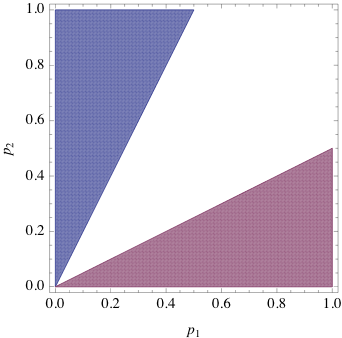
\includegraphics[width=2.2in]{Figure1a} & & 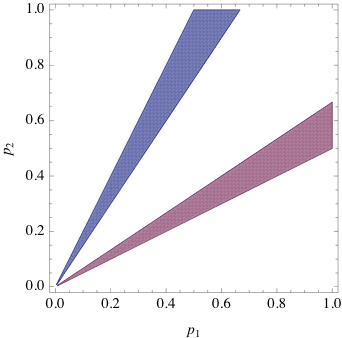
\includegraphics[width=2.2in]{Figure1b} \end{tabular}
 (c)
 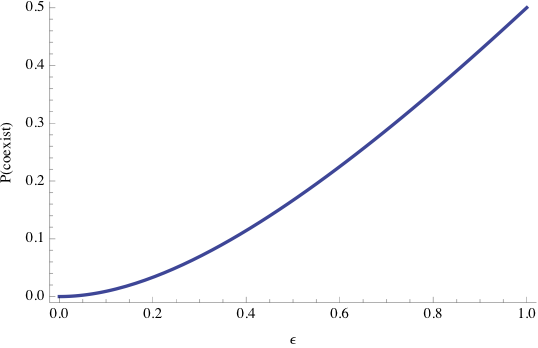
\includegraphics[width=4in]{Figure1c}
   \caption{The regions of coexistence for two species are plotted in $p$-space. (a) shows the coexistence regions for $\epsilon=1$ while the case $\epsilon=1/2$ is shown in (b). Shaded regions in the upper left half of the plot are where both species coexist with growth rates $p_1<p_2$, or equivalently trait values $x_1>x_2$. The  regions to the bottom right of the plots represent the alternative ordering $p_1>p_2, x_1<x_2$. (c) shows how the probability of coexistence increases with the asymmetry parameter $\epsilon$, with large values indicating strong competitive asymmetry between individuals of different trait values.}
 \label{fig:2d}
\end{figure}

Since the trait values are limited to a finite range, it is possible to calculate the probability of coexistence for two species chosen at random from a uniform distribution on $x_1,x_2 \in [0,1]$  by calculating the size of the area within the unit box $[0,1]^2$ which satisfies \eqref{2dcond} as well as the assumption $x_1>x_2$. Here, we first find the area in $p-$space for which there exists an interior fixed point, and then from that calculate the area in $x-$space. Since $p$ is a decreasing function satisfying $p(0)=1, p(1)=0$, it is invertible with increasing inverse $p^{-1}$ that satisfies $p^{-1}(1)=0, \, p^{-1}(0)=1$, and hence the range of $p^{-1}$ is $[0,1]$. We first find the area in the $p_1,p_2$ plane, writing $p_i=p(x_i)$ for simplicity of notation, for which
\begin{equation}
\label{2dcond2}
\frac{p_2}{1+\epsilon}>p_1>p_2(1-\epsilon),\;\; (p_1,p_2)\in [0,1]^2,
\end{equation}
and then map this to an area in $x_1,x_2$ space.


Since the case $p(x_i)=1-x_i$ is linear and maps $[0,1]^2$ onto itself, the probability of coexistence is equal to the area of the $x-$space satisfying (\ref{2dcond}) which in turn equals the area in $p-$space satisfying (\ref{2dcond2}).

The areas satisfying these conditions for $\epsilon=1$ and $\epsilon=1/2$ are shown in Figure~2. To calculate the size of the area in the $p_1,p_2$ plane where both equilibrium populations are greater than zero, we note that when \eqref{2dcond2} intersects the unit box, it forms a triangle $T$ with vertices $(0,0),(1-\epsilon,1)$ and $(1/(1+\epsilon),1)$. The area of $T$ in the $p_1,p_2$ plane is therefore given by
\[
\frac{1}{2}\left(\frac{1}{1+\epsilon}-(1-\epsilon)\right)=\frac{\epsilon^2}{2(1+\epsilon)},
\]
which is then multiplied by two to account for the other ordering of trait values $p_2<p_1$ (i.e. $x_2>x_1$) to give the area as
\[
A =\frac{\epsilon^2}{1+\epsilon}.
\]
This area is an increasing function in $\epsilon$, meaning that the greater the asymmetry observed in the competition between species, the more likely it is that two species can coexist together, as anticipated by our numerical simulations of the concave-convex function and analytical work on the piecewise linear function. Note that the result here is identical to that when $\Theta$ is small in the piecewise linear case.

 
\subsubsection{Communities with $n$-species}
In communities with $n>2$ species present,  any interior fixed point is unique and globally stable. While Nowak and May \cite{nowak1994superinfection} state that this result holds with a modification of the theory in Chapter 21.3 of \cite{hofbauer1998evolutionary}, we include our own proof in Appendix~\ref{appendix1c}. 

In order to find the region of trait space that permits an interior fixed point, we consider the model written in the form
\begin{equation}
\frac{dN_i}{d\tau}=N_i\left(p_i(x) - \sum_{j=1}^n c_{ij}(x)N_j\right),
\end{equation}
where the $c_{ij}(x)$ competition coefficients combine to give the competition matrix $C(x)$. In Appendix~\ref{appendix1d}, we show that the volume of coexistence can be calculated from a determinant and is given explicitly by
\[
V_{n}=
\left\{
\begin{array}{rl}
\frac{\epsilon^{n}}{(1+\epsilon)^{n-1}} & \mbox{ even }n\geq 2\\
\frac{\epsilon^{n-1}}{(1+\epsilon)^{n-1}} & \mbox{ odd }n\geq 3. 
\end{array} \right.
\]
Therefore, for all $0<\epsilon \leq1$, it is possible for any number $n$ of species to coexist along a single competition-fecundity trade-off. However it is increasingly difficult for all species to coexist as the number of species in the environment increases, as shown by Figure~3.

\begin{figure}[htbp]
   \centering
   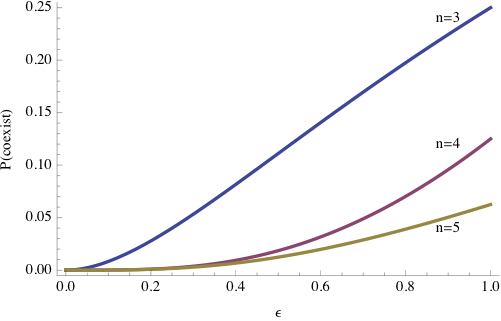
\includegraphics[width=4in]{Figure3}
   \caption{How the probability of coexistence for different numbers $n$ of species decreases with $n$ is shown, along with how it changes with $\epsilon$, shown for $n=3,4,5$ species coexistence}
   \label{fig:ndif}
\end{figure}


\section{Discussion}

Life-history trade-offs have a rich history in helping to explain how competitors may coexist, but relatively few studies have quantified how rapidly the likelihood of coexistence declines with increasing number of species within the community. Here we have considered a trade-off between competitive ability and fecundity and have shown the probability of multiple species coexistence depends critically on the degree of asymmetry $\epsilon$ between them. Large values for $\epsilon$ indicate large competitive asymmetry between species with even nearby trait values, and it is here that coexistence is found to be most likely (see Figure~3). However, as the number of species drawn from the pool increases, even small decreases in the competitive asymmetry can lead to rapid declines in the likelihood of coexistence. The probability of sustaining at least two species also depends on the slope of the competition function at $c(z=0)$, and this is determined by the parameter $\Theta$. As $\Theta$ decreases, the steepness of the competition curve increases, and so does the probability of the trade-off maintaining multiple species. Therefore, maximum coexistence is likely to be achieved at high $\epsilon$ and low $\Theta$.

The trade-off considered here is essentially the same as the competition-colonisation trade-off, which has been much studied theoretically (e.g.  \cite{levin1974disturbance, hastings1980disturbance, tilman1994competition}) and empirically (e.g. \cite{turnbull1999seed, robinson1995invasibility, cadotte2007competition}). Although early theory suggested any number of species might be able to coexist on this trade-off \cite{may1994superinfection, tilman1994competition}, as we have shown here, coexistence is dependent upon the steepness of the trade-off function, and also on the amount of asymmetric competition between the species. Recent theory that builds on this trade-off has shown that high levels of coexistence are possible on a tolerance-fecundity trade-off, where species with seeds that can tolerate wide ranges in environmental conditions are assumed to be larger, and therefore fewer in number \cite{muller2010tolerance}. However, this still invokes strong competitive asymmetry because smaller seeded species are unable to germinate in environments outside of their tolerance zone, and it is probable that even some ability to germinate in non-preferred patches might greatly reduce the amount of coexistence that is possible.

Our results connect  to the results of Adler and Mosquera \cite{adler2000space}, who showed the shape of the trade-off to be important for the number of species that can coexist; and with HilleRisLambers and Dieckmann \cite{hillerislambers2003competition} who found strong trade-offs tend to enhance the coexistence of two species sharing one resource. We have extended this work to consider how rapidly the area for coexistence in trait-space diminishes with the number of species in the community. Our analyses reveal that even with the trade-off assumptions that most favour coexistence, the likelihood of coexistence diminishes very rapidly with the number of species, and this suggests relatively few species are ever likely to be able to coexist on one trade-off. Moreover, our results reveal that competitive asymmetry becomes more important in generating coexistence as the number of species increases (Figure~3; equation \eqref{nspecies}).

The methods we use are similar to those of Meszena et al \cite{meszena2006competitive} who calculated the likelihood of an interior fixed point existing and it's dependence on their model parameters. However, we note the existence of an interior fixed point is not sufficient for coexistence. For example, the symmetric May-Leonard model for three species \cite{may1975nonlinear}, always admits an interior equilibrium, yet the system only exhibits permanence when for each species, intraspecific competition is greater than twice the sum of the interspecific effects of the other two species. As such, their model represents an upper bound to the likelihood of coexistence. In the current paper, we address this by proving that the existence of an interior equilibrium is exactly equivalent to the permanence of the system, therefore adding to the conclusions made by Meszena et al.

Our results therefore show how important competitive asymmetry is in generating and maintaining large numbers of coexisting species; but how prevalent is competitive asymmetry in natural communities? There is a large body of work to suggest competitive asymmetry is common in animal (e.g. \cite{lawton1981asymmetrical, morin1988experimental,  resetarits1995competitive, costanzo2005asymmetrical}) and plant communities (e.g. \cite{weiner1990asymmetric, connolly1996asymmetric, keddy1997experimental}). However, to our knowledge, except for seed size variation in plants (e.g. \cite{turnbull1999seed}), this competitive asymmetry has rarely been connected to a life-history trade-off. It is worth noting that many of these studies consider only two species, and the competition coefficients are often measured under one set of environmental conditions, so it is not clear how much this asymmetry extends into large communities of competitors, and whether there is a temporal fluctuation in the competitive hierarchy. One exception to this is a study by Keddy et al. \cite{keddy1997experimental} who measured the competitive asymmetry between pairs of plant species drawn from a pool of 18 species. Their work concluded that in fact competitive asymmetry increased with soil productivity, and this is because light rather than soil nutrients became the limiting factor, and generally competition for light is expected to be size asymmetric, whereas competition for soil nutrients is usually size symmetric (e.g. \cite{weiner1990asymmetric}). 

The model we analyse here is biologically rather simple, and there is much scope for extensions that incorporate more realism. For example, as for most other models that study the competition-fecundity or competition-colonisation trade-offs, we assume that intraspecific competition is identical for all trait values (equation (\ref{rescaledmodel})); but it might be more realistic to assume that smaller individuals are better able to share resources than larger individuals, meaning the intraspecific competition term now has to be trait dependent as well.  We believe relaxing this assumption would yield rather more complex dynamics than the current model, including the possibility of founder control (i.e. unstable interior equilibria). For example, Calcagno et al. \cite{calcagno2006coexistence} incorporated priority effects, whereby an adult plant cannot be displaced be a seed, into a competition-colonisation model, and showed that this can actually increase coexistence. However, when maximum colonisation rate, analogous to our maximum population growth rate, is heavily limited, such preemptive competition generally ceases to be beneficial to coexistence. Therefore,  this would reduce the amount of coexistence compared to that found here, and would place greater dependence on multiple trade-offs or other processes to generate coexistence between large numbers of species. 

The models presented here have assumed linear intrinsic growth rate $p$ in the absence of competition, and linear or piecewise constant competition for communities with three or more species. Nonlinearity, with suitable monotonicity conditions, can be easily incorporated into the function $p$, and the volume in $x-$space can then be found through a change of variable in the volume integral. Moreover, changing $p$ does not impact on the globally stability of interior steady states, which, as shown, depends solely on the competition matrix $C$. For models with three or more species, studying nonlinear competition functions gives the difficulty of not only finding volumes in space enclosed between curved surfaces, but also determining which points in these volumes are globally stable. The alternative, focusing on coexistence measured by permanence, also presents a serious challenge due to the lack of necessary and sufficient conditions for permanence in general competitive Lotka-Volterra models for $n>3$.

These extensions aside, we have shown here that competitive asymmetry could be very important in maintaining several species on a single trade-off; but that for large numbers of species multiple trade-offs; and/or other processes such as disturbance or natural enemies are required to maintain diverse competitive communities. Nonetheless, it is clear that competitive asymmetry which is widely observed in empirical studies could still interact with these other processes to increase, rather than decrease biodiversity as has often been supposed (e.g. \cite{keddy1997experimental, resetarits1995competitive}).

\section*{Acknowledgement}

Thanks to the reviewers for their comments. This work was funded by a Natural Environment Research Council (NERC) studentship to SN.

\section*{Appendices}
\bappendix
\section{Effect of the slope $c'(0)$ on coexistence}
\label{appendix1a}
We note that since $c(z)+c(-z)=2$ constant, we have that $c(-z)-1=1-c(z)>0$for positive $z$. Therefore, we can subtract \eqref{x2lower} from \eqref{x2upper} to get
\[
\frac{(1-z-c(z))-((1-z)c(-z)-1)}{c(-z)-1}=\frac{z(c(-z)-1)}{(c(-z)-1)}=z.
\]
Therefore the upper and lower bounds for $x_2$ coincide at $z=0$, and for $z>0$ the upper bound is always greater than the lower, i.e there is always a region where coexistence is possible. Therefore, if the upper bound \eqref{x2upper} is non-increasing, both it and the lower bound \eqref{x2lower} never exceed the value they achieve at $z=0$, and there is only a region of coexistence in the positive quadrant when the limit
\[
\lim_{z \to 0}\frac{1-z-c(z)}{1-c(z)} >0.
\]
As both numerator and denominator tend to zero, we use l'Hopital's rule to get that this limit is given by
\[
\frac{-1-c'(0)}{-c'(0)}
\]
which is positive for $c'(0)<-1$.

It remains to demonstrate that \eqref{x2upper} is non-increasing for positive $z$. The derivative of the function is given by
\[
\frac{c(z)-1-zc'(z)}{(1-c(z))^2}.
\]
If $c'(z)=0$, then this becomes
\[
\frac{-1}{1-c(z)}<0, \]
since $c(z)<1$ for all $z>0$. When $c'(z)<0$, then we note that the function is non-increasing for 
\[
z\leq \frac{c(z)-1}{c'(z)}.
\]
The derivative of the right hand side is given by
\[
1-\frac{c''(z)(c(z)-1)}{c'(z)^2}
\]
which is greater than one for all positive $z$. Therefore, this point increases faster than $z$. Noting that the derivative of \eqref{x2upper} is zero when $z=0$, we can therefore conclude that for all $z>0$, this upper bound is indeed non-increasing.

\section{The absence of asymmetry}
\label{appendix1b}
Without losing any generality, we can order traits such that $x_1>x_2 > \cdots > x_n$ so that since $p$ is decreasing, $p(x_1)< p(x_2) < \cdots < p(x_n)$. When $\epsilon=0$, equations \eqref{rescaledmodel} become
\[
\frac{d N_i}{d\tau}=N_i\left(p(x_i)-\sum_{j=1}^n N_{j}\right), \;\; i=1,\ldots,n.
\]
Thus if $i < k$,
\[
\frac{d}{d\tau} \log (N_i/N_k) = p(x_i)-p(x_k)<0.
\]
This shows that for $i<k$
\[
N_i(\tau) = N_k(\tau) e^{( p(x_i)-p(x_k)) \tau} \rightarrow 0, \;\; \tau\rightarrow \infty
\]
since $N(t)$ is bounded. This shows that $N_{i}(\tau)\rightarrow 0$ as $\tau\rightarrow \infty$ for $i=1,2,\ldots,n-1$. It is intuitive that the remaining species density $N_n(\tau) \rightarrow p(x_n)$ as $\tau\rightarrow \infty$. This can be shown by first noting that the equation for the dynamic of $N_n$ reduces to  the time-dependent logistic equation:
\begin{equation}
\dot{N}_n = p(x_n) N_n \left(1-\frac{N_n}{K(t)}\right), \label{ss1}
\end{equation}
where the time-dependent carrying capacity is given by 
\[
K(t) = p(x_n)e^{p(x_n)t}/(\sum_{i=1}^n e^{p(x_i)t}).
\] One may verify that the explicit solution to (\ref{ss1}) is
\[
N_n(t) = \frac{N_n(0) e^{p(x_n)t}}{1+N_n(0)\sum_{i=1}^n \left( \frac{e^{p(x_i)t}-1}{p(x_i)} \right)}\rightarrow p(x_n)\mbox{ as } t\rightarrow \infty.
\]
We have thus shown that the species with minimum trait $0$ will send any other species to extinction.

\section{Global Stability of interior fixed points}
\label{appendix1c}
\begin{lem}Whenever an interior fixed point exists for the $n$-species model given by \eqref{rescaledmodel}, it is both unique and globally asymptotically stable relative to the interior of the region of space where all $N_i$ are positive, and therefore the system displays permanence.\end{lem}
\begin{proof} It is well known that when \eqref{model} admits an interior steady state, it is globally stable (also known as LV-stable) if the  matrix $-C=((-c_{ij}(x)))$ is dissipative, that is, there exists a positive diagonal matrix $D$ such that the real symmetric matrix $D(-C)+(-C)^TD$ is negative definite, and therefore has only negative eigenvalues (e.g. \cite{hofandsig}). For the model with discontinuous competition,  the competition matrix takes the form (in the region $x_1>x_2>\cdots > x_n$) given by equation (\ref{constant_C}). 
Let $D$ be a positive diagonal matrix with diagonal entries $\theta_i$ ($i=1,\ldots,n$).
Then \eqref{model}, with competition matrix $C$ as in \eqref{constant_C}, admits a  fixed point that globally attracts interior trajectories whenever the real symmetric matrix $A=(DC+C^TD)$, given by
\[
\label{posdef}
\begin{pmatrix}
2\theta_1&(1-\epsilon)\theta_1+(1+\epsilon)\theta_2&\cdots&(1-\epsilon)\theta_1+(1+\epsilon)\theta_n\\
(1-\epsilon)\theta_1+(1+\epsilon)\theta_2&2\theta_2& \cdots&(1-\epsilon)\theta_2+(1+\epsilon)\theta_n\\
(1-\epsilon)\theta_1+(1+\epsilon)\theta_3&(1-\epsilon)\theta_2+(1+\epsilon)\theta_3&\cdots&(1-\epsilon)\theta_3+(1+\epsilon)\theta_n\\
\vdots&\vdots&\ddots&\vdots&\\
(1-\epsilon)\theta_1+(1+\epsilon)\theta_n&(1-\epsilon)\theta_2+(1+\epsilon)\theta_n&\cdots&2\theta_n
\end{pmatrix} 
\]
has all positive eigenvalues, which is the case if all the leading principal minors are positive.

We have fixed $\theta_i>0$ positive, so we restrict ourselves to looking at $m\times m$ leading principal minors of the matrix $A$ with $m\geq2$:
\[
 \begin{vmatrix}
2\theta_1 & (1-\epsilon)\theta_1+(1+\epsilon)\theta_2 & \cdots & (1-\epsilon)\theta_1+(1+\epsilon)\theta_m \\
(1-\epsilon)\theta_1+(1+\epsilon)\theta_2 & 2\theta_2 &\cdots & (1-\epsilon)\theta_2+(1+\epsilon)\theta_m \\
\vdots&\vdots&\ddots&\vdots \\
(1-\epsilon)\theta_1+(1+\epsilon)\theta_m & (1-\epsilon)\theta_2+(1+\epsilon)\theta_m &\cdots & 2\theta_m \end{vmatrix}. 
\]
As the determinant of a matrix is not changed when one row or column is subtracted from another, we then subtract the $(m-1)$th column from the $m$th column, and the $i$th column from the $(i+1)$th column for all $1\leq i\leq m-1$ to obtain the matrix
\[
 \begin{vmatrix}
2\theta_1 &(1+\epsilon)(\theta_2-\theta_1) & \cdots &(1+\epsilon)(\theta_m-\theta_{m-1}) \\
(1-\epsilon)\theta_1+(1+\epsilon)\theta_2 & (1-\epsilon)(\theta_2-\theta_1) &\cdots & (1+\epsilon)(\theta_m-\theta_{m-1}) \\
\vdots&\vdots&\ddots&\vdots \\
(1-\epsilon)\theta_1+(1+\epsilon)\theta_m & (1-\epsilon)(\theta_2-\theta_1) &\cdots & (1-\epsilon)(\theta_m-\theta_{m-1}) \end{vmatrix}. 
\]
Removing the common factors in columns 2 up to $m$ give that the determinant has a factor
\[
(-1)^{m-1}\prod_{i=1}^{m-1}(\theta_i-\theta_{i+1})
\]
which is then multiplied by
\[
\begin{vmatrix}
2\theta_1 & 1+\epsilon & 1+\epsilon & \cdots & 1+\epsilon \\
(1-\epsilon)\theta_1+(1+\epsilon)\theta_2&1-\epsilon&1+\epsilon&\cdots&1+\epsilon \\
(1-\epsilon)\theta_1+(1+\epsilon)\theta_3&1-\epsilon&1-\epsilon&\cdots&1+\epsilon \\
\vdots&\vdots&\vdots&\ddots&\vdots \\
(1-\epsilon)\theta_1+(1+\epsilon)\theta_m&1-\epsilon&1-\epsilon&\cdots&1-\epsilon \end{vmatrix}.
\]
Subtracting row $m-1$ from row $m$, and row $i$ from row $i+1$ for all $i<m$ gives this determinant as
\begin{align}
&\begin{vmatrix}
2\theta_1 & 1+\epsilon&1+\epsilon&\cdots&1+\epsilon \\
(1+\epsilon)(\theta_2-\theta_1)&-2\epsilon&0&\cdots&0 \\
(1+\epsilon)(\theta_3-\theta_2)&0&-2\epsilon&\cdots&0 \\
\vdots&\vdots&\vdots&\ddots&\vdots \\
(1+\epsilon)(\theta_m-\theta_{m-1})&0&0&\cdots&-2\epsilon \end{vmatrix} \notag \\
=&\begin{vmatrix}
2\theta_1&1+\epsilon&0& 0&\cdots&0\\
(1+\epsilon)(\theta_2-\theta_1)&-2\epsilon&2\epsilon &0&\cdots&0\\
(1+\epsilon)(\theta_3-\theta_2)&0&-2\epsilon&2\epsilon&\cdots&0\\
\vdots&\vdots&\vdots&\vdots&\ddots&\vdots \\
(1+\epsilon)(\theta_m-\theta_{m-1})&0&0&0&\cdots&-2\epsilon\end{vmatrix}\notag \\
=&(-1)^{m-1}\theta_12^m\epsilon^{m-1} - (1+\epsilon)^2(2\epsilon)^{m-2}(-1)^{m-2}\left(\theta_2-\theta_1+\theta_3-\theta_2+\dots+\theta_m-\theta_{m-1}\right)\notag \\
=&(-1)^{m}(2\epsilon)^{m-2}\left( (1-\epsilon)^2\theta_1-(1+\epsilon)^2\theta_m\right). \notag
\end{align}
Therefore, the $m\times m$ leading principal minor for $m>1$ is given by
\begin{equation}
-(2\epsilon)^{m-2}\left( (1-\epsilon)^2\theta_1-(1+\epsilon)^2\theta_m\right)\prod_{i=1}^{m-1}(\theta_i-\theta_{i+1}). \label{baig1}
\end{equation}
It remains to be shown that the $\theta_i$ can be chosen such that all leading principal minors (\ref{baig1}) are positive, which is the case when $\left( (1-\epsilon)^2\theta_i-(1+\epsilon)^2\theta_j\right)<0$ and $(\theta_i-\theta_j)>0$ for $i<j$. Setting
\[
\theta_i=n-\frac{1}{(1+\epsilon)^{n+1-i}}
\]
then we can use $j-i\geq1$ to calculate that
\begin{align}
\theta_i-\theta_j=&\left(n-\frac{1}{(1+\epsilon)^{n+1-i}}\right)-\left(n-\frac{1}{(1+\epsilon)^{n+1-j}}\right) \notag \\
=&\frac{(1+\epsilon)^{j-i}-1}{(1+\epsilon)^{n+1-i}} \notag \\
\geq&\frac{1+\epsilon - 1}{(1+\epsilon)^{n+1-i}}>0. \notag
\end{align}
To show that $\left( (1-\epsilon)^2\theta_i-(1+\epsilon)^2\theta_j\right)<0$ we note that
\begin{align*}
\left( (1-\epsilon)^2\theta_i-(1+\epsilon)^2\theta_j\right)&<\left( (1-\epsilon)^2\theta_1-(1+\epsilon)^2\theta_j\right)\\
&<\left( (1-\epsilon)^2\theta_1-(1+\epsilon)^2\theta_n\right)
\end{align*}
and that for $\epsilon=0$, we have $\left( (1-\epsilon)^2\theta_1-(1+\epsilon)^2\theta_n\right)=0$. Differentiating this with respect to epsilon gives
\begin{align*}
\frac{d}{d\epsilon}\left( (1-\epsilon)^2\theta_i-(1+\epsilon)^2\theta_j\right)&=-4n+1+2\frac{1-\epsilon}{(1+\epsilon)^n}+n\frac{(1-\epsilon)^2}{(1+\epsilon)^{n+1}}\\
&\leq-4n +1+2+n < 0
\end{align*}
for all $0\leq \epsilon \leq 1$ and $n\geq2$. Therefore, since $\epsilon=0$ is a root for the function, for any $\epsilon>0$, we have
$$\left( (1-\epsilon)^2\theta_1-(1+\epsilon)^2\theta_n\right)<0$$
and therefore
$$\left( (1-\epsilon)^2\theta_i-(1+\epsilon)^2\theta_j\right)<0.$$
Therefore, all the leading principal minors are positive, meaning that $A=DC+C^TD$ is positive definite. Therefore $D(-C)+(-C)^TD$ is negative definite, as required for global stability. Global stability immediately implies permanence. \begin{flushright} $\square$ \end{flushright}
 \end{proof}
 
 \section{Size of the coexistence region}
 \label{appendix1d}
Here we calculate the probability of coexistence for an $n$ species version of \eqref{rescaledmodel}. Since we are using the step function \eqref{stepc}, the matrix $C(x)$ is piecewise constant. At the interior fixed point the bracketed terms are equal to zero, which therefore reduces the model to
$
\mathbf{p}(x)=C(x)\mathbf{N},
$
with $\mathbf{p}$ the vector of the growth rate of each species and $\mathbf{N}$ the vector with $i$th component $N_i$. Since $C(x)$ is non-singular, this is the rearranged to give the solution 
$
\mathbf{N}=C^{-1}(x)\textbf{p}(x)$. 
We are interested in the volume of $x$-space for which $\mathbf{N}=C^{-1}(x)\mathbf{p}(x)> \mathbf{0}$. To find this volume, we find the volume in $p$-space where $p_1 < p_2 <\cdots < p_n$ which satisfies, since then $x_1>x_2> \cdots > x_n$ and so $C(x)$ is a constant, and non-singular matrix $C$, so that
\begin{equation}
C^{-1}\mathbf{p} = \mathbf{0}. \label{planes1}
\end{equation}
Equation \eqref{planes1} defines a series of planes in $p-$space that all pass through the origin. When an ordering $p_n>p_{n-1}>\dots>p_1$ is assumed without any loss of generality, these planes form an $n$ dimensional pyramid when intersected with the unit cube. The volume of this pyramid is then the probability of the $n$ species model permitting an interior fixed point, and therefore the probability of all $n$ species coexisting due to the stability result in Appendix~\ref{appendix1c}.

With the ordering $p_1<p_2<\dots<p_n$, equivalent to $x_1>x_2>\dots>x_n$, the competition matrix $C$ takes the form
\begin{equation}
\label{constant_C}
C=\begin{pmatrix}
1 & 1-\epsilon &1-\epsilon & \cdots & 1-\epsilon \\
1+\epsilon&1&1-\epsilon&\cdots&1-\epsilon \\
1+\epsilon&1+\epsilon&1&\cdots&1-\epsilon \\
\vdots&\vdots&\vdots&\ddots&\vdots \\
1+\epsilon&1+\epsilon&1+\epsilon&\cdots&1 \end{pmatrix}.
\end{equation}
It is relatively simple to show that $C$ is non-singular, allowing us to calculate the volume of the $n$ dimensional pyramid. We need to find the $n$ points at which $n$ of the planes intersect the face $p_n=1$. To find these points, we note that the edges of the $n$ dimensional pyramid must be orthogonal to each of the $n-1$  planes in $p-$space defined by \eqref{planes1} that meet at that edge. Since $C^{-1}C=I_n$, each column of $C$ is orthogonal to all bar one of the rows of $C^{-1}$ Therefore, the edges of the $n$ dimensional pyramid point in the direction of the columns of $C$. These edges meet the plane $p_n=1$ at the non-zero corners of the $n$ dimensional simplex, so it is simple to show that these points are given by the columns of $C$, scaled such that the value of $p_n=1$. Therefore, the $n$ non-zero vertices of the  simplex that lie in the plane $p_n=1$ are given by
\begin{gather*}
\left(\frac{1}{1+\epsilon},1,1,1,\dots, 1\right), \\
\left(\frac{1-\epsilon}{1+\epsilon}, \frac{1}{1+\epsilon}, 1, 1,\cdots, 1\right), \\
\left(\frac{1-\epsilon}{1+\epsilon}, \frac{1-\epsilon}{1+\epsilon},\frac{1}{1+\epsilon}, 1,\cdots, 1\right), \\
\vdots \\
\left(\frac{1-\epsilon}{1+\epsilon}, \frac{1-\epsilon}{1+\epsilon},\frac{1-\epsilon}{1+\epsilon},\cdots, \frac{1}{1+\epsilon},1\right), \\
\left(1-\epsilon, 1-\epsilon,1-\epsilon,\cdots, 1-\epsilon,1\right).
\end{gather*}
\begin{thm} the  probability of coexistence, is given by
\begin{equation}
\label{nspecies}
V_n=P(\text{coexist}_n)=\begin{cases}
\frac{\epsilon^n}{(1+\epsilon)^{n-1}} &  \mbox{ even }n\geq 2 \\
\frac{\epsilon^{n-1}}{(1+\epsilon)^{n-1}} &   \mbox{ odd }n\geq 3 \end{cases}.
\end{equation} \end{thm}
\begin{proof}
The volume of the $n$ dimensional simplex  is given by 
\[
\bar{V}_n=\frac{1}{n!}\begin{vmatrix}
\frac{1}{1+\epsilon}&1&1&1&\cdots &1&1\\
\frac{1-\epsilon}{1+\epsilon} & \frac{1}{1+\epsilon} & 1& 1& \cdots &1&1\\
\frac{1-\epsilon}{1+\epsilon} & \frac{1-\epsilon}{1+\epsilon}& \frac{1}{1+\epsilon} & 1& \cdots &1&1\\
\vdots&\vdots&\vdots&\vdots&\ddots&\vdots\\
\frac{1-\epsilon}{1+\epsilon} & \frac{1-\epsilon}{1+\epsilon}& \frac{1-\epsilon}{1+\epsilon} & \frac{1-\epsilon}{1+\epsilon}& \cdots &\frac{1}{1+\epsilon}& 1\\
1-\epsilon & 1-\epsilon & 1-\epsilon & 1-\epsilon& \cdots & 1-\epsilon & 1
 \end{vmatrix}.
\]
Since there are $n!$ of these volumes, one for each ordering of the traits, so the total volume is $V_{n} = n! \bar{V}_n$. Let $U_n = n! (1+\epsilon)^{n-1}\bar{V}_n$. Then 
\[
U_n=\begin{vmatrix}
1&1+\epsilon&1+\epsilon&1+\epsilon&\cdots &1+\epsilon&1+\epsilon\\
1-\epsilon& 1 & 1+\epsilon& 1+\epsilon& \cdots &1+\epsilon&1+\epsilon\\
1-\epsilon &1-\epsilon&1 & 1+\epsilon& \cdots &1+\epsilon&1+\epsilon\\
\vdots&\vdots&\vdots&\vdots&\ddots&\vdots\\
1-\epsilon&1-\epsilon&1-\epsilon&1-\epsilon& \cdots &1& 1+\epsilon\\
1-\epsilon& 1-\epsilon &1-\epsilon &1-\epsilon& \cdots &1-\epsilon& 1
 \end{vmatrix}.
\]
We now show that $U_n = \epsilon^2  U_{n-2}$. To see this, first subtract the second row from the first row. Having done this, in the new determinant subtract the first column from the second column. This gives
 \[
U_n=\begin{vmatrix}
\epsilon & 0 &0&0&\cdots &0&0\\
1-\epsilon& \epsilon & 1+\epsilon& 1+\epsilon& \cdots &1+\epsilon&1+\epsilon\\
1-\epsilon &0&1 & 1+\epsilon& \cdots &1+\epsilon&1+\epsilon\\
\vdots&\vdots&\vdots&\vdots&\ddots&\vdots\\
1-\epsilon&0&1-\epsilon&1-\epsilon& \cdots &1& 1+\epsilon\\
1-\epsilon& 0 &1-\epsilon &1-\epsilon& \cdots &1-\epsilon& 1
 \end{vmatrix},
\]
which gives $U_n = \epsilon^2 U_{n-2}$ as required. Now quick calculations show that $U_2=\epsilon^2$ and $ U_3 = \epsilon^2$ so that $U_n = \epsilon^n$ for $n\geq 2$ even and $ U_n = \epsilon^{n-1}$ for $n\geq 3$ odd.
 \begin{eqnarray*}
\bar{V}_{n} &=& \frac{1}{n!} \frac{\epsilon^n}{(1+\epsilon)^{n-1}} \mbox{ $n$ even}\\
 &=&\frac{1}{n!}\frac{\epsilon^{n-1}}{(1+\epsilon)^{n-1}} \mbox{ $n$ odd.}
 \end{eqnarray*}

\[
V_{n}=
\left\{
\begin{array}{rl}
\frac{\epsilon^{n}}{(1+\epsilon)^{n-1}} & \mbox{ even }n\geq 2\\
\frac{\epsilon^{n-1}}{(1+\epsilon)^{n-1}} & \mbox{ odd }n\geq 3. 
\end{array} \right.
\]   
\end{proof}

\eappendix
